\chapter{Description of the Word2Vec Model }
\label{chap:word2vec_description}


\section{Introduction}
Continuous space language  models
learned by a neural network have
demonstrated good results across a variety of tasks in the field of \ac{NLP}.  As pointed out by
the authors, these continuous word vector representation achieves a level of
generalization not possible with class traditional $N$-gram based models
\cite{conf/icassp/MikolovKBGC09}. In addition to the language model itself,
the word vector representations are learned in the initial layers of the
\ac{NN}. These 
induced representations  have been used successfully to improve the
performance of existing \ac{NLP} tasks \cite{collobert:2008}
\cite{Turian:2010:WRS:1858681.1858721}. 

As discussed in section \ref{sec:mikolov-neural-net-model},  one of the way to learn a
\ac{NNLM} is to learn the word vectors using  a \ac{NN} with a single hidden
layer. Then, these word vectors are used to  train another \ac{NN}, in this 
way obtaining   the final \ac{NNLM} \cite{conf/icassp/MikolovKBGC09}.   
What is particular about this architecture is that they learn the  word
vectors without  even constructing the complete language model.  This means
that in practice,  the two step can be performed separately \cite{conf/icassp/MikolovKBGC09}. 

This chapter describes in detail a recent approach to efficiently learn
high-dimensional word representation \cite{DBLP:journals/corr/abs-1301-3781}.
In other words, focusing only on the first part of the previously described 
architecture. It has been found that the word vectors learned in this manner,
not only capture linguistic regularities of words  but also semantic
relationships. As the word vector generated from this architecture is used 
through this work, it is necessary to describe this particular model with more
detail.

% making it  necessary to describe
%%it properly.  
The rest of the chapter is structured as follows: section
\ref{sec:word2v-generalities} gives a general description of
\textit{Word2vec}.  Section \ref{sec:word2v-architectures} and
\ref{sec:word2v-tran-algorithms} describe in more detail the available
architecture and training algorithms. Finally, section
\ref{sec:w2v_other_paramters} describe additional  parameters that
directly affect the generated learned representations.

% \section{Modern Neural Network Language Model Architectures}

% In order to understand  \textit{Word2vec}'s it is necessary to study the
% models on which it is built upon. Word2vec as both an improvement and
% as well as a simplification of a full-fledged \ac{NNLM}.
% Therefore, this section introduces
%briefly the most common  architectures and their more important
%characteristics.

% \subsection{Model Complexity}

% One of the main reason behind the development of \textit{Word2vec} was the
% need of obtaining good word vector representation with low training complexity cost.

% A neural probabilistic language model

% Note that Bengio [1] claims that training word features
% together with neural network language model is better than
% independent training of features and n-gram NN LM. In our
% approach, we consider the first network as a feature extractor
% and do not train it together with the n-gram net. We suppose
% that this can prevent word features from learning cache-like
% relationships in the data, which tend to heavily optimize per-
% plexity, but not recognition accuracy (Goodman [8]).


\section{Word2vec Generalities}
\label{sec:word2v-generalities}

\textit{Word2vec} is an open source project released in 2013 by the Tomas
Mikolov,  Kai Chen, Greg Corrado, and Jeffrey Dean.  
Its overall architecture has been described in several paper published at the
time of its release
\cite{DBLP:journals/corr/abs-1301-3781,MikolovSCCD13,conf/naacl/MikolovYZ13} 
and some previous work \cite{mikolovphd2012}. The source code, sample corpus
and the dataset used to evaluate the quality of the word vectors  can be downloaded freely from the project's
 web page\footnote{http://https://code.google.com/p/word2vec/}.
\textit{Word2vec}'s architecture
has its origin  in the architecture described back in section 
\ref{sec:mikolov-neural-net-model} where a \ac{NNLM} is learned separately. 
First learning the word representation using a \ac{NN} and then learning then
estimating equation (\ref{eq:lm_probability}) using a $N$-gram neural
network.  \textit{Word2vec} in that sense, it  is a simpler model, as it  does not
try to learn the full probability distribution as a full \ac{NNLM} does.
Instead, it  focuses on learning good representations of words by  only
performing  the first step  of the aforementioned architecture. %  In that sense, it is an
% unsupervised feature learning algorithm.

As  described in section \ref{sec:nnlms-intro}, the complexity of all 
these models arises from the non-linear layers  that allows the \ac{NN} to
obtain complex representations.  \textit{Word2vec} removes the additional
hidden layer  allowing it to be trained efficiently on much more data  \cite{DBLP:journals/corr/abs-1301-3781}.

\textit{Word2vec} is not a single architecture or model, it is formed by a
group of related architectures, learning algorithms, optimization 
approaches and some tricks. The combination of all these characteristic
allows the model  to learn word representation in a efficient
way. It has been shown that these representations  capture semantic and
syntactic 
similarities as mean of vector offsets, allowing the model to answer complex
semantic and syntactic questions by means 
of simple vector operations   \cite{MikolovSCCD13}. This property  has also
been used to perform word vector based translation \cite{DBLP:journals/corr/MikolovLS13}.  

A model trained with \textit{Word2vec}  can be characterized by the following properties:


\begin{itemize}
\item \textbf{Architecture}: Skip-gram or \ac{CBOW}.
\item \textbf{Training Algorithm}: hierarchical softmax  or \ac{NEG}.
\item \textbf{Additional paramters}: Discussed in section \ref{sec:w2v_other_paramters}
\end{itemize}


Table \ref{tab:word2_vec_parameters} summarizes the most important parameters
that need to be selected at training time
and affect the resulting word vector representations. Then comment column is
taken from the description  on the project web page.


\begin{table}[h]
   \centering
   \caption{Summary model training parameters} 
   \label{tab:word2_vec_parameters}
   
   \small
   \begin{tabular}{ |l|c|p{5cm}| }
   \hline           
    Parameter &  Possible Values & Comment \\  \hline           
    \multirow{2}{*}{Architecture}  & skip-gram  & Slower, better for frequent
    words. \\ 
    \cline{2-3}
    & \ac{CBOW}  &  Faster than skip-gram. \\ \hline
    \multirow{2}{*}{Training Algorithm}  & Hierarchical Softmax  & Better for infrequent words.   \\ 
    \cline{2-3}
    & \ac{NEG} & Better for frequent works \\ \hline
    Sub-sampling  & 1e-3 to 1e-10  &  It  can improve both accuracy and speed for large data
    sets Useful values are in range \\ \hline
    Dimensionality  & 10-640 & Higher dimension the better results. 
    it depends on data availability.  \\ \hline
    Context (Window size)  & 5 - 15 & The number of word used to predict. \\ \hline

    
\end{tabular}
\end{table}

% What is word 2 vec ... !
% Summary of the model
%% Architecture
%% Algorithm
%% Other important parameter
%%% Subsampling
%%% Window

\section{Word2vec Architectures}
\label{sec:word2v-architectures}


\subsection{Continuous Bag of Word (CBOW) Architecture}

This architecture is similar in spirit to the  \ac{FNNLM} described in section
\ref{subsec:fwd-neural-net-lm} were a context of $n$ is used. However with two main differences. First the
non-linear hidden layer is removed and second the projection layer is shared for
all words (not just the projection matrix of word vectors). This means that
all the words are projected to the same position and their vector averaged.
% Another difference with the presented \ac{FNNLM}  is that words from future are used. 
The training criterion is to correctly classify the middle word of a window
of $N$ that is used per train cycle. That is both word from the past and the
future are used to predict the word in the center of a sentence. 


\begin{figure}[hptb!]
    \centering
    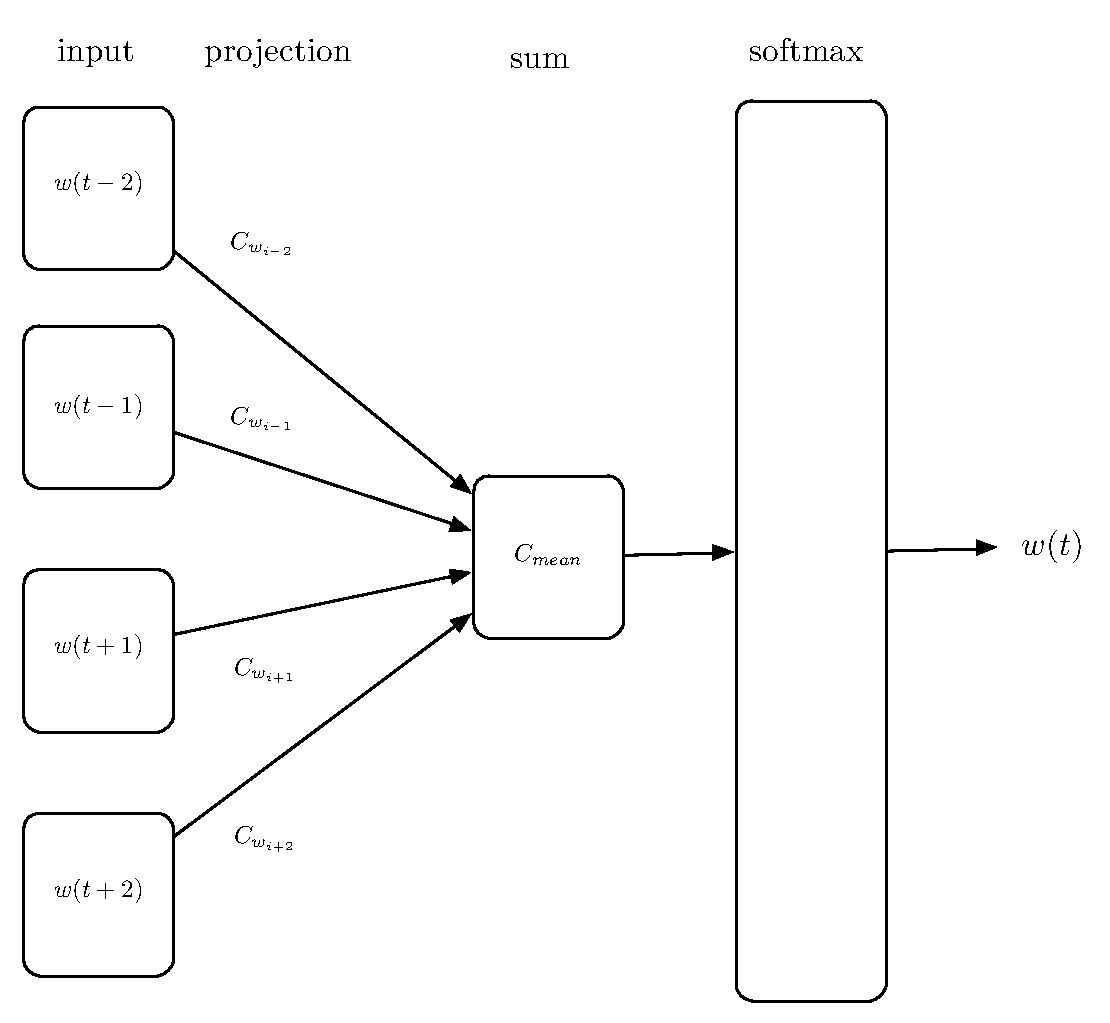
\includegraphics[width=0.6\textwidth]{images/word2vec-cbow-latex.pdf} 
    \caption{CBOW Architecture}
    \label{fig:cbow-architecture-alone}
\end{figure}

More formally, given a sequence of words with 1-of-$K$ representation $w_1,w_2,w_3, \dots, w_T$ and a window
of size $n$. Defining $C_m(t)$ as:

\begin{equation}
\label{eq:cbow-mean}
   C_{m}(t) =    \frac{\sum_{-n \leq j \leq n, j \neq 0} { 
       C_{w_{t+j}}} } {2n}    
\end{equation}

The  objective  \ac{CBOW}  ties to maximize the average log probability:


\begin{equation}
  \label{eq:logprob-cbow}
   \frac{1}{T} \sum^{T}_{t=1} \text{log} \, p
     \left( w_t \, |\, C_{m}(t) \right),
\end{equation}



With the probability  $p\left( w_O \, |\, v \right)$  defined as:

\begin{equation}
  \label{eq:logp-cbow}
  p(w_O|v) = \frac{\text{exp}\left(C^{'}_{w_o}\,^\top\,v \right)
  }{\sum^{V}_{w=1} \text{exp} \left( C^{'}_w \,^\top\, v \right)   }  
\end{equation}


Where $C_w$ and $C^{'}_w$ are the input representation (the weights from the input layer to the
projection layer) and output representation (the weights from
projection layer to the softmax layer) respectively.   Figure
\ref{fig:cbow-architecture-alone} shows a graphical representation of
\ac{CBOW} architecture.

Similarly as other \ac{NNLM}s, the complexity of this architecture
is defined by its structure:

\begin{equation}
  Q = N \times D + D \times  log_2(V)
\end{equation}

Assuming a for of hierarchical softmax is used to efficiently calculate the
probability distribution, as described for all the \ac{NNLM}s in section \ref{sec:nnlms-intro}.


\subsection{Skip-Gram Architecture}
\label{sec:skip-gram-architecture}

The Skip-gram architecture is similar to \ac{CBOW}, but it instead of
predicting the current word based on the context, it tries to maximize
classification of a  word based on another word on the same sentence
\cite{DBLP:journals/corr/abs-1301-3781}.  Each  word is used as input
to the \ac{NN} that  predicts words within certain range before and after 
it (i.e. it tries to predict the surrounding words or context). 
\cite{DBLP:journals/corr/abs-1301-3781}. Figure
\ref{fig:skipgram-architecture-alone} show depicts this approach graphically.


\begin{figure}[hptb!]
    \centering
    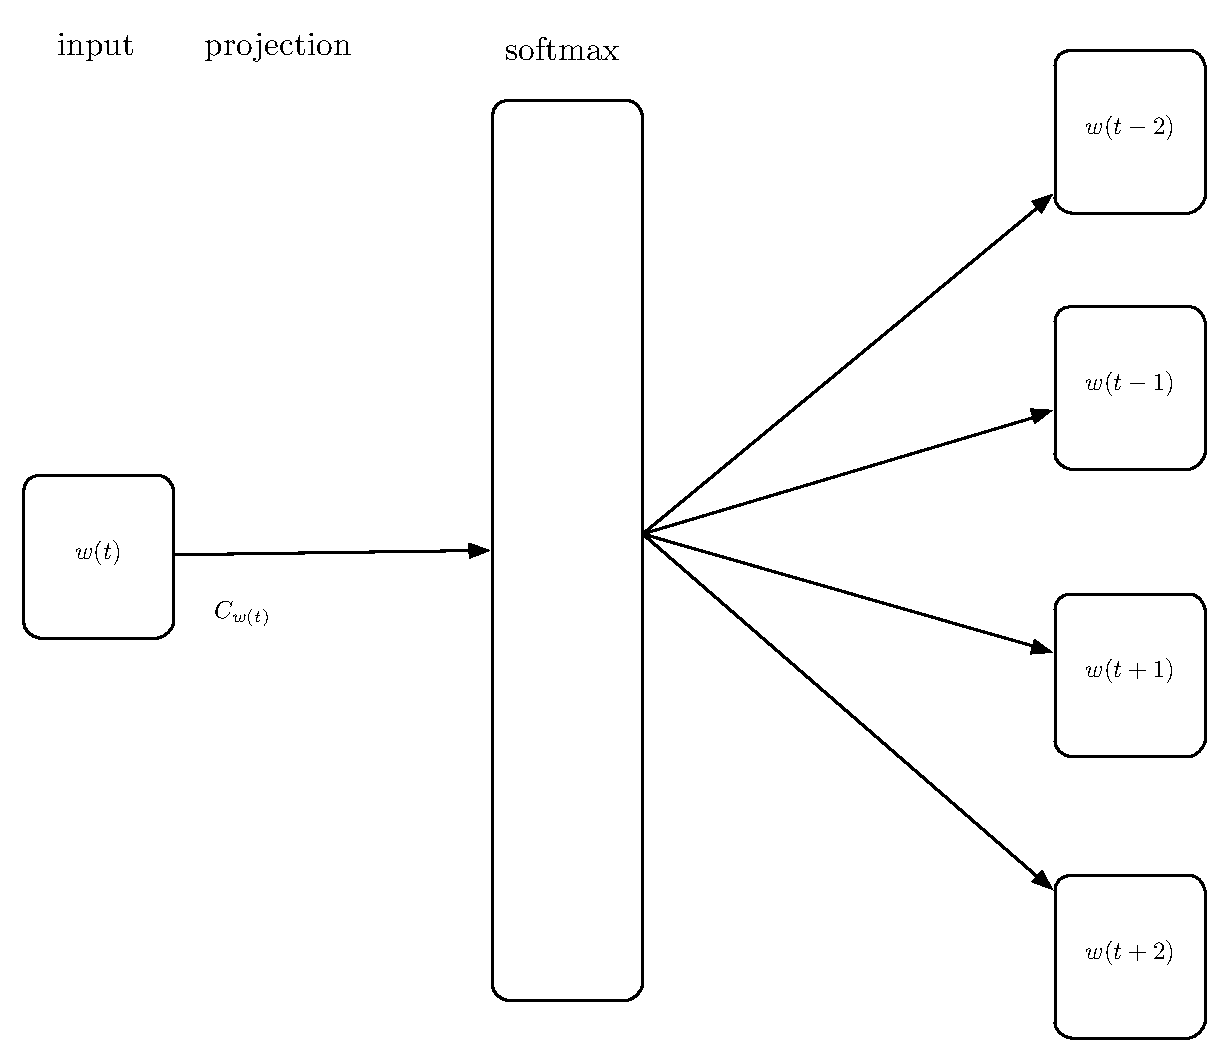
\includegraphics[width=0.6\textwidth]{images/word2vec-skipgram-latex.pdf} 
    \caption{The Skip-gram architecture. The current word $w(t)$ is used to
      predict the  surrounding words.}
    \label{fig:skipgram-architecture-alone}
\end{figure}



Similarly to  \ac{CBOW}, if a sequence of training words $w_1,w_2,w_3,
\dots, w_T$ is given, the probability to maximize is give by

 \begin{equation}
  \label{eq:sumprob-cbow}
   \frac{1}{T} \sum^{T}_{t=1}{\sum_{-r \leq j \leq r, j \neq 0}\text{log} \, p
     \left( w_{t+j} \, |\, w_t  \right)}
\end{equation}

with $r$ is the size of the window, i.e. the training context is $2r$.
Increasing this range improves quality of the resulting word vectors but it
also increases the computational complexity.

Using the softmax function the probability  $p(w_O|w_I)$ is given by:

\begin{equation}
  \label{eq:logp-skgram}
  p(w_O|w_I) = \frac{\text{exp}\left(C^{'}_{w_O}\,^\top\,C_{w_I} \right)
  }{\sum^{V}_{w=1} \text{exp} \left( C^{'}_w \,^\top\, C_{w_I} \right)   }  
\end{equation}


Where $C_w$ and $C^{'}_w$  has the same meaning as in the \ac{CBOW}
formulation,  and $V$ is the number of words in the vocabulary.

The training complexity of this architecture is proportional to
\cite{DBLP:journals/corr/abs-1301-3781}:

\begin{equation}
  Q = R \times (D + D \times log_2 \left(V)\right),  
\end{equation}

Where R is the maximum distance of words. A random number $r$ in the range $<
1; R >$ is selected. Then, $r$ words from the history and $r$ words from future are used as the correct labels for the current word.
 

\section{Word2vec Training Algorithms}
\label{sec:word2v-tran-algorithms}
Another one of the principal  characteristics of  \textit{Word2vec} is the
available training algorithms. In
fact, the selection of the training algorithm has a large  impact on
 the quality of the learned vector representation,  and in the
computational performance.

The formulations for calculating $p(w_i|v)$ and  $p(w_O|w_I)$  ( equations
(\ref{eq:logp-cbow})  and  (\ref{eq:logp-skgram}) ) are impractical because
the cost of computing them is proportional to $V$, which is often large.
Therefore, computational efficient alternatives need to be devised in order to
train this model in real world data sets. Here when the training algorithms
come into play, as they are alternative to this computationally expensive
calculation. 

\subsection{Hierarchical Softmax}
\label{sec:sub-hs}


An efficient alternative to calculating the full softmax is the hierarchical
softmax. In the context of \ac{NNLM}s, it was first introduced by Morin and
Bengio \cite{Morin05hierarchicalprobabilistic}. Hierarchical softmax is more
computationally efficient that a normal softmax layer because instead of
evaluating output nodes $V$ (i.e. each of the words on the output layer) to
obtain the probability distribution, it only needs to evaluate about
$\text{log}_2 \left( V \right)$ nodes \cite{MikolovSCCD13}.

This is achieved by  using a binary tree to represent the output layer with
the $V$ of the vocabulary as its leaves, for each node, explicitly represent
the relative probabilities of its child nodes. Previous work reports several
strategies to create the binary tree \cite{Mnih08ascalable}, all of them with
different effects on the performance. The authors of \textit{Word2vec} use a
Huffman Tree  to represent the hierarchical softmax.

To build the tree, the probabilities are calculated beforehand just counting
each occurrence of  the word in the text 
and diving it by the total number of words (the unigram probability).  With these probabilities, the
Huffman codes are calculated \cite{huf52}, and thus the tree is built. The
words with high probabilities get shorter codes ending up on top tree. As the
probabilities of the child nodes can be obtained from its parent,  it is not
necessary to visit all then children but just take it from that node. Figure
\ref{fig:huffam-tree-w2v-example} shows a example of a how this Huffman tree
would look if created from a imaginary and  highly unlikely corpus. 


% Use this to generate the initial graphviz file: http://huffman.ooz.ie/


\begin{figure}[h]
    \centering
    \caption{Huffman tree in \textit{Word2vec example}}
    \label{fig:huffam-tree-w2v-example}
\end{figure}

More precisely, the tree is used as follows: each word $w$ is reached by an
appropriate path from the root of the tree (i.e. the Huffman code). Let
$n(w,j)$ be the $j$-th node on the path from the root to $w$, and let $L(w)$
be the length of this path. So $n(w,1) = \text{root}$ and $n(w,L(w)) = w$. In
addition, for any inner node $n$, let $ch(n)$ be an arbitrary fixed child of
$n$ and let $[\![ x ]\!] $ be 1 if $x$ is true and -1 otherwise. Then the
hierarchical softmax defines the $p(w_O|w_I)$  by \cite{MikolovSCCD13} : 


\begin{equation}
   \label{eq:hierarchical-softmax-prob}
  p(w_O|w_I)  = \prod^{L(w)-1}_{j=1}\sigma\left( [\![n(w,j + 1) = ch(n(w,j))   ]\!] \cdot C^{'}_{n(w,j)}  \,^\top\, C_{w_I}   \right) 
\end{equation}
Where $\sigma(x) = 1/(1 + \text{exp}(-x)) $.  Thus the cost of computing the
log-probability and the gradient is proportional to $L(w_O)$ which for a
binary tree is not greater than $\text{log}_2(V)$.   $C_{w_{I}}$ is again the
representation  of word $w_{I}$  but   $  C^{'}_{n(w,j)}
$ is the projection of the node $n$ on the tree.  So the the number of output
nodes is also  approximately $\text{log}_2(V)$. A equivalent model replacing
$C_{w_I}$ by $v$ is easily constructed for the \ac{CBOW} architecture.

\subsection{Negative Sampling}

An alternative to the hierarchical softmax is \ac{NCE}, which was  introduced in the
context of language model by Mnih and Teh \cite{citeulike:4416856}. \ac{NCE}
is in turn based in the concept of importance sampling, which use a known
distribution to try to approximate the gradient based on samples not from the
original distribution $p(w_t) $ but from a known distribution $q(x)$ easy to
sample from.  In other words, instead of fitting the density model, it is
learned to classify from samples of the data distribution and samples from a
noise distribution $q(x)$ that is already know. 
As the objective of \textit{Word2vec} is not to learn a language model but
useful representation, so authors simplified  to the original \ac{NCE} and
defined an  alternative formulation named \ac{NEG}: 

\begin{equation}
  p(w_O|w_I)  =  \text{log}\,\sigma\left(C^{'}_{n(w,j)}  \,^\top\, C_{w_I}
  \right) + \sum^{k}_k\mathbb{E}_{w_{i}\sim P_{n}(w)}\left[
    \text{log}\,\sigma\left(-C^{'}_{w_i}  \,^\top\,  C_{w_I} \right)  \right]
\end{equation}

The main difference between this approach and \ac{NCE}  needs both
samples and the numerical probabilities of the noise distribution, while \ac{NEG} uses only
samples \cite{MikolovSCCD13}.  Equivalently to  hierarchical softmax, a formulation from  the \ac{CBOW}
 architecture can be constructed by replacing the appropriate variables.
In the \textit{Word2vec} implementation, the
noise distribution  $P_n(w)$ is the unigram distribution $U(w)$ raised to the
$3/4rd$. This was selected by the authors empirically given that outperformed
other alternative distribution such as the unigram and the uniform
distribution. 



\section{Other Parameters}
\label{sec:w2v_other_paramters}
This section describes the additional paramters needed by the model and that
affect the quality of the word vectors.


\subsection{Dimension }
\label{sec:w2v-param-dim}
Perhaps the most important parameter after the architecture and the training
algorithm is the dimension of the learned word vector.  This parameter define
the projection layer size. Generally speaking the larger the better.
However, in order to benefit from a larger dimension size, more data need to
be used, as it  reaches a upper bound based on the availability of the data.
The author of \textit{Word2vec} report dimension from 100 to 640 on the
largest dataset used. This, as it was just mention is corpus dependent.


\subsection{Window}
\label{sec:w2v-params-win}

An important parameter that need to be defined at training size is the
\textit{window} or context size. Generally speaking the context size is two
times the window. More formaly, the context $R(w_i)$ comes from a window of
size $r$ around the word:

\begin{equation*}
R(w_i) =
w_{i-k},\ldots,w_{i-1},w_{i+1},\ldots,w_{i+k},
\end{equation*}

In  the \ac{CBOW} architecture, the window defines the number of words used to
calculate the continuous bag of word ( equation (\ref{eq:cbow-mean}).  For
the Skip-gram architecture, the window defines  the number of words that the
$w_i$ needs to predict from a sentence.  Generally speaking,  larger
context generally provide better word representation but at expense of
computation time. The window  is generally set empirically its  will depend
on the grammatical structure of the source language of the corpus used and the task at hand.


\subsection{Subsampling of Frequent Words}
\label{sec:sub-hs}

In large corpora the most frequent words occur many times (e.g.
``in'', ``at'', ``the'', etc.). These words  provide  less information value
than other rare words  \cite{MikolovSCCD13}.  \textit{Word2vec} discards a
word $w_i$ in the training set with a probability computed by the formula:

\begin{equation}
  \label{eq:w2v-subsampling}
  P(w_i)= 1 - \sqrt{\frac{t}{f(w_i)}}
\end{equation}
where $f(w_i)$  is the frequency of word $w_i$ and t is a threshold that can
be specified  by the user at training time. The subsampling of words also
affect indirectly the size of the window. In addition to the subsampling
paramter, \textit{Word2vec} offer a parameter called 
\textit{min-count} which discards all the words that appear less than a
number of times in all the corpus.   As the subsampling and the removal of
\textit{min-count} words occur  \emph{before} the actual context creation,
the actual effective window size increase. These include words that are
content-full and linearly far from the word in focus, therefore making the similarities more topical.


\section{Evaluation of the Word Representation}
\label{sec:w2v-evaluation-word-repr}

In their original paper \cite{DBLP:journals/corr/abs-1301-3781}, the authors
introduced a comprehensive test that contained five types of semantic
questions. In the original dataset  there were 8869 semantic and 10675
syntactic questions. To create this set the authors compiled a list of
similar word pairs manually and then they generated the list by
connecting the word pairs. Table~\ref{tab:task_original_en} shows examples 
examples from each category of tasks. 

To evaluate the quality of the word vectors the question  are answer in the
following manner: given the word pairs ($a$, $b$) and ($c$, $d$) a question
is considered to be answered correctly if the for resulting vector $X$ the closest vector measured in
cosine similarity is  $vector(d)$. $X$ is calculated by applying the following
operation $X = vector(b) - vector(a) + vector(c)$.  Given two vectors $A$ and $B$, the
cosine similarity is calculated in the following way: 

$$\text{similarity} = \cos(\theta) = {A \cdot B \over \|A\| \|B\|}$$


 For example  for the words
($``small''$, $''smaller''$ ) and ($''big''$ ,$"bigger"$),
the $vector("bigger")$ should be the closest to the resulting
vector $X$. If the representation of the word in
vector space is good, then it is possible to find the answer using such
operation \cite{DBLP:journals/corr/abs-1301-3781}.

As discussed in the first part of this work, the word representations
capture different types of  similarities among words. Therefore, with the
operation described above,  what is  being
attempted is to answer the question ``\emph{What is the word that is similar to
c in the same sense as b is similar to a?}''. 

\renewcommand{\arraystretch}{1.3}

\begin{table}[h]

  \centering
  \caption{Examples of the original types of syntactic questions in the
    Semantic-Syntactic Word Relationship test as defined 
    by \cite{DBLP:journals/corr/abs-1301-3781}. }
  \label{tab:task_original_en}
  \small
  \begin{tabular}{ |l| |c|*{4}{c| |c| c | c }  }

  \hline           
  Type of Relationship &  \multicolumn{2}{c||}{Word Pair 1} &
  \multicolumn{2}{c|}{Word Pair 2} \\  \hline           
  Common capital city & Athens & Greece & Oslo  & Norway \\ 
  All capital cities  & Astana & Kazakhstan &  Harare & Zimbabwe  \\
  Currency & Angola & kwanza & Iran & rial \\  
  City-in-state  & Chicago & Illinois & Stockton & California \\  
  Man-Woman & brother & sister  & grandson & granddaughter \\  \hline  
  Adjective to adverb & apparent & apparently & rapid & rapidly  \\  
  Opposite & possibly & impossibly & ethical & unethical \\  
  Comparative & great & greater & tough & tougher \\  
  Superlative & easy & easiest & lucky & luckiest \\  
  Present participle & think & thinking & read & reading \\  
  Nationality adjective & Switzerland & Swiss & Cambodia  & Cambodian  \\  
  Past tense & walking & walked & swimming & swam \\ 
  Plural nouns  & mouse & mice & dollar & dollars \\  
  Past verbs & work & works & speak  & speaks  \\  \hline  
\end{tabular}
\end{table}


\section{Conclusion}
\label{sec:sub-w2v-desc-conclusion}
\textit{Word2vec} allow to train word vector representations from  large
corpus of text in a efficient way. The vector  representations  capture semantic and
syntactic relationship, relationships that can be explored via simple vector
operations. In this chapter we described the  architecture, algorithm and techniques
behind it.  There are two main differences between \textit{Word2vec} and a traditional \ac{NNLM}, first
it does not care to estimate the actual probability of  a next word given a
previous context, but only of obtaining good representation. In that sense
\textit{Word2vec} is not a  language model, but a feature learning algorithm.  Second, it uses
words not only from the past, as more traditional language models do, but
also from the future, allowing the model learn complex relationships among
words.  Finally, it is not a deep architecture. In fact, the architecture only
contains a layer. This, among other things allows it efficiently train
representations that are useful to improve existing \ac{NLP} tasks.



%define the number of words  from the past and from the 
% y. This formulation is impractical because the cost of computing
% ∇ logp(wO|wI) is proportional to W, which is often large (105–107
% terms).

% Huffman coding is an entropy  encoding algorithm used for lossless data
% compression.  It was developed by David A. Huffman while he was a Ph.D.
% student at MIT. \cite{huf52}.

% Huffan cioding is an algorithm to proce an  optimal symbol code $C$ for a given 
% \emph{pmf} $ p = (p_1,....,p_n) $.  Huffman coding builds a tree orderded by frequency.



%%% Local Variables: 
%%% mode: latex
%%% TeX-master: "../main.tex"
%%% End: